\chapter{Background}
\label{ch:back}
\section{Context of the project}
\label{sec:back:context}
Before discussing the research method we employ for the remainder of this thesis we will attempt to focus our efforts by scoping the project. This will be achieved by two analyses. First we will attempt to describe the set of target applications in more abstract concepts. Secondly we will focus our efforts be defining the stakeholders that stand to gain from an implementation of the intended monitoring platform. 

\subsubsection*{Defining the set of applications}
%TODO kleine ref van c/v analysis van architecture
As stated before the concrete group of target applications for the QoS monitoring platform is WSN and IoT applications. However we can scope the group of applications more conceptually by specifying and parametrizing the data emitted by them and expected after processing, since this will be the input and output data for our platform and its implementations. For the purpose of scoping we will consider an implementation-agnostic  of the platform as a black box. In doing so we can focus on the intended inputs and expected outputs, and their contrasts, without concerning the internals of the platform to be designed.

Firstly we have the issue of \emph{individual information capacity}. Individual messages emitted by applications and presented to the platform contain very little individual capacity for information. Some information can be extrapolated from it, but only about the device that emitted it and at the exact moment the measurements were taken. Though, for example, detection of failure of a single node is an important task, it probably has little impact on the application at large if this application concerns thousands of sensors. This immediately identifies a second feature of the emitted data, in that it is extremely multi-source. The data originates from an incredible amount of distributed devices. This entails that, though the measured data-points from similar devices describe similar data, the aggregation of data from these sources is not a trivial task. Not only is a series of data temporally relevant, it is also related across the plain of topologically distributed sensor devices. Finally the huge amount of devices and the dynamic nature of sensor networks and IoT induces a high degree of (dynamic) scalability. Therefore any back-end application --- main processing or auxiliary support --- should anticipate and provide a sufficient potential for scalability. In contrast we have the expectations of the outcomes of the platform. Firstly, the platform is expected to output a relatively small amount of high-information actions, alerts and reports. The high-information consequences directly contradict the low-information capacity of individual device messages. Conversely, the moderately small number of output responses/events contradicts the immense influx of data-messages into the platform. These contradictions in turn affect the required scalability of the platform. 

The transformation from low individual information capacity to high information messages can be achieved through three means. the first is enrichment, which uses outside sources to annotate and amend the data in a device measurement message (e.g. device location data extracted from a server-side database)\cite{data_enrichment}. The second is transformation, which takes raw low-level datapoints and performs calculations on them to transpose it to higher-level information (e.g. combining location data and time to calculate the speed of an object)\cite{information_transformation}. The third method is data aggregation and reduction. This method joins and merges related datapoints accross several --- and often vast amounts of --- input messages to formulate a single output message containing a few datapoints, depicting some collective parameters of the domain \cite{information_transformation}. Again the reach of this domain can be temporally, geographically, et cetera. The first two methods operate on individual data entries emitted by sensors. Hence they can be easily parallellized and are thus increadibly scalable \cite{boek:Exploratory Data Mining and Data Cleaning:C3}. However the aggregation implies an eventual reduction into a single snapshot on a single machine. This introduces possible single points of failures or congestion, and if adequate precautions are not taken scalability is lost.

To summarize, the input data is characterized by \emph{low individual information value}, \emph{multi-source} and \emph{extremely high volumes}. Conversely the output is characterized by a \emph{finite} number of \emph{high information value} whose data processing will require \emph{scalable data enrichment and aggregation}. This will be the parameters of the scope of applications observed by the platform and the successive applications the platform will serve.

\subsubsection*{Stakeholder analysis}
Another approach to scope our efforts is by identifying the stakeholders for our platform. We will perform this by analogy of the Onion Stakeholder Model as proposed by [ref]\cite{onion}. This model divides stakeholders in consecutive layers, ordered by the degree of interaction and benefits received from the product. For the stakeholder division we will consider the product to be both the platform to be developed and potential future implementations of the platform. Intuitively, this project definition would result in a two level product in the model, with the platform as core and the group of all instantiations al the first layer around it. However since this analysis focusses on human stakeholders, we will treat it as a single instance in our application of the model. A visual representation of the application of the onion model is given in Figure \ref{fig:onion}.

The first layer of the model directly encasing the product is \textbf{Our System}. It encompasses the designed and developed product (i.e. the platform and its instances) and the human parties that directly interface with the product. The first group of these stakeholders is the \emph{Employee Developing and Maintaining} implementations of the platform. They interact directly with scaffolding and frameworks provided by the core platform. Some explanations of the onion model place developers in the outer layer of the model (the wider environment), since after development they no longer interface with the product unless they remain involved in a maintenance capacity. However, since developers of a platform instantiation interact with the scaffolding and frameworks directly provided by the core platform, we emphasize their importance by placing them in the system layer of the model. The second role in the system layer is the \emph{Normal Operator}. These operators receive information from the product directly and interact with subsequent systems and operational support employees to effect change. For our product this entails changes to the application under investigation or reports regarding the long term performance of the application to be forwarded to managers and employees higher up in the organization.

The second layer of the model is the \textbf{Containing System}. It contains stakeholders that are heavily invested in the performance and benefits of the product, but do not interact with it directly on a regular basis. We have identified two of these stakeholder roles. The first is the \emph{Support and Maintenance Operator} of the application observed by the platform. If we were to analyse the stakeholders of the application under investigation, these operators would be placed in the first layer of the model. However since they do not (necessarily) directly interface with our support platform, they are placed in the second layer of the model for our product. They are however heavily invested in the performance and results of the platform, since identified problems and deficiencies can direct their efforts toward maintaining and improving their own application. The second role in this layer is the \emph{Sales Person} of the application under investigation. Again this regards a sales person of the application under investigation, not our support platform. The task of a sales person is to convince potential clients to employ a developed product. Performance guarantees are an important part of a sales pitch held by this type of stakeholder. Therefore employees of sales departments benefit hugely from known, concrete and stable QoS metrics.

The third layer of the model is the \textbf{Wider Environment}. This final layer contains stakeholders that do not sentiently interface with the product and are not heavily or conciently interested in its execution or performance, but are affected by it to some degree. The first stakeholder role in this category is the \emph{Financial Benefactor}. This entity is not heavily invested in the development and dayly routine of the system, but does benefit financially from it. This role applies to investors, companies and other business units that are not concerned with the technical upkeep of the product, but do benefit from the gained revenue or cost-efficient measures provided by the product. Closely related with this is the \emph{Political Benefactor}. This benefactor does not directly reap monetary benefit from the solution, but does gain political benefit from it. This can apply to both stakeholders in public office or private business by improving their position in their respective markets. The final stakeholder is the \emph{General Public}. Members of the public do not interface with our platform in any capacity, but can benefit heavily from it. For example, many WSN and IoT applications are deployed in smart city management and industry4.0\cite{voorbeelden}. Though deployment of dependable IoT technologies in these fields require initial investments, in the long term these technologies can improve efficiency, reducing costs and prizes. Therefore, guaranteed uptime and low resource usage can benefit the consumer, without them realizing it. Though the benefit to singular consumers are relatively small, due to the huge size of the public at large this amounts to a incredible benefit.

\begin{figure}
\centering
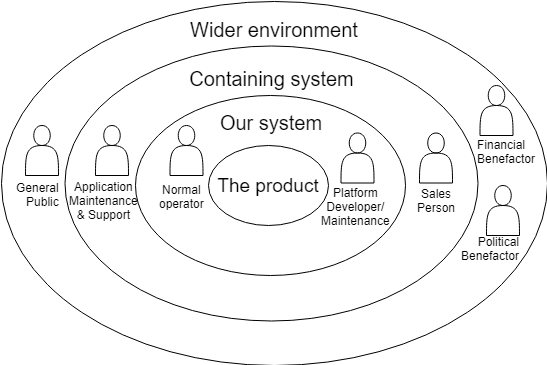
\includegraphics[width=.7\textwidth]{resources/img/onion.png}
\caption{Visual depiction of application of onion stakeholder model}
\label{fig:onion}
\end{figure}
\section{Micro-service architecture}
%TODO write
\section{Quality of Service \& Quality of Information}
%TODO afkortingen?
%TODO write
\subsection{Quality of Service in WSN} 
Existing platforms?
\subsection{WSN energy conservation methods} 
\subsection{Quality of Information of WSN data}
\label{sec:back:qoi}
Aside from Quality of Service, in WSNs and IoT applications we find the concept of Quality of Information (QoI). QoI [describes] parameters depicting quality attributes of information presented by and derived from as system. It is especially [applicable] to WSNs as they present raw low-level which is then highly processed by subsequent applications. We will therefore employ the concept of QoI to validate and evaluate the processing architecture presented in chapter \ref{ch:architecture}.

%TODO cite or parafrase
\cite{qoi_definition} identifies the following attributes describing Quality of Information.
\begin{description}
\nospace
\item[Accuracy] The degree of correctness which provides the level of detail in the deployed network. It is the value which is the close imitation of the real world value.
\item[Precision] The degree of reproducibility of measured values which may or may not be close (accurate) to real world value.
\item[Completeness] The characteristic of information which provides all required facts for user during the construction of information.
\item[Timeliness] An indicator for the time needed when the first data sample is generated in the network till the information reaches the target application for decision making.
\item[Throughput] The maximum information rate at which information is provided to the user after raw data collection.
\item[Reliability] The characteristic of information, in which information is free from change or no variation of information from the source to the end application.
\item[Usability] The ease of use of information that is available after raw data collection has undergone processing and can be applied to the application based on user's evolvable requirements.
\item[Certainty] The characteristic of information from the source to the sink with desired level
of confidence helping the user for decision making.
\item[Tunability] The characteristic of information, where the information can be modified and undergo processing based on user's evolvable requirements.
\item[Affordability] The characteristic of information to know the cost for measuring, collecting and
transporting the data/information. It is the expensiveness of information. 
\item[Reusability] The characteristic of information, where the information is reusable during its lifetime or as long as it is relevant.
\end{description}
\section{Constraint programming and solving paradigms}
\label{sec:back:constraint}
In chapter \ref{ch:rdm} we will visit the concept of constraint programming and solvers. The concept of constraint programming encompasses modelling a problem by means of a collection of correlated variables and associated value domains. The relations between variables are captured in a list of constraints. The problem is then solved by finding assignments for each variable with respect to their domains which conforms with the specified constraints. 

An example of a problem modelled as constraint problem is an automatic sudoku solver. The model would be a list or matrix of integer variables, with each entry having a domain $\{V_i|1\leq V_i\leq 9\}$. The constraint we would have is $V_1 \neq V_2$ for every combination of entries $(V_1,V_2)$ in the same row, column or 3-by-3 grid .

Several methods exist in order to solve a combinatorial constraint problem. The first and simplest is to perform a brute force search over the solution space. This would produce the cartesian product of the domains of all variables ($\prod_{i\in I} D_i$) and test them against the constraints. Candidate solutions are rejected until a valid composition of variable assignments is found. This is however a very inefficient procedure as it has to search though the entire search space without optimization. For large combinatorial problems this search space grows exponentially. For our sudoku example for instance we find that if 20 values are predetermined, then our solution space has a size of $9^{61}(\approx 1,6\cdot 10^{58})$.

A more efficient search algorithm is presented by backtrack search. Whereas the brute force approach assigns every variable a value and then checks its validity, the backtrack search algorithm operates on a subset of the variables assigned. By incrementally assigning values to variables it performs a systematic Depth First Search through the search space. If a partial assignment is determined to violate the set of constraints, the algorithm will reject the entire remainder of the search tree. In this manner the algorithm optimizes failing variable assignments by attempting to identify them earlier. For the example of the sudoku solver this entails that an assignment of a 3 to a position adjacent to another square with a 3 will immediately halt the exploration of that branch of the search tree, without the need to consider subsequent variable assignments. It will instead backtrack through the tree by rolling back assignments and attempt a different assignment.

The backtrack search algorithm can be improved upon further by implementing constraint propagation. This technique attempts to prune invalid variable values from the domain before they are assigned by the backtrack search algorthm. For example if a square in the sudoku is assigned a three, then the effect of this assingment will be propegated by pruning the number 3 from the domains of every entry in the same row, column or 3-by-3 grid. This eliminastes inconsistent options that would violate the constraints befere they would be assigned. Additionally, the concept of local inconsistency can be extended to variable domains without reequiring any assingment. For example if we have two variables $V_1$ and $V_2$ with domains $D_1=\{1,2,3\}$ and $D_2=\{2,3,4\}$ and the constraint $V_1 \geq V_2$, then the values 1 and 4 can be pruned from $D_1$ and $D_2$ respectively since they are inconsistent with any of the values in the oppoising domain and can therefore never validate the constraint. \cite{constraint_general, constraint_algorithm}
\section{Design Methods}
\subsection{Commonality/variability analysis}
\label{sec:back:cv_analysis}
In order to design for our problem domain it will require conceptualization. We will conceptualize the problem domain(s) by means of a commonality/variability analysis (C/V analysis). Whereas this analysis is [usually] performed during the process of system decomposition in product line engineering, it can also be employed to identify common and varying concepts in a problem domain. \cite{cva_problem_domain}.  This analysis identifies the common concepts - or invariants - that may be assumed fixed and may be depended upon and the variations in the problem domain which will need to be [captivated] and accounted for by our solution.

\cite{cv_analysis} describes the process of a commonality/variability analysis in five steps.

\begin{enumerate}
\nospace
\item Establish the scope: the collection of objects
under consideration.
\item Identify the commonalities and variabilities.
\item Bound the variabilities by placing specific on each variability.
\item Exploit the commonalities.
\item Accommodate the variabilities.
\end{enumerate}

In our conceptualization of the problem domain we will mostly focus on step 2 in which we will provide a list of common definitions, shared commonalities and variabilities. Also, in our approach we will combine steps 4 and 5 by formulating a list of requirements for our solution based on the identified commonalities and accounting for the found variabilities. As the list of requirements depends on invariants and accommodates variabilities it will allow us to design automated solutions.

\subsection{Design Science Methodology}
\label{sec:back:dsm}
%TODO write
\section{Example case}
\label{sec:example_case}
Throughout this [thesis] we will demonstrate our solutions by applying them to a hypothetical case. Though this case may sometimes seem oversimplified and nonsensical, it does provide an elementary example to illustrate all facets of our solutions without overcomplicating the case. This case is expressly not intended to demonstrate the capabilities or utility of our proposed solution. For that purpose, an application to a more complex real-world case will be performed in section \ref{ch:validation}. 

The case we propose encompasses an enormous network of low power devices sensing for meteorologically anomalous events. These sensors perform measurements on a regular interval and transmit the measurements to a cell tower to be forward to a back-end application for further processing. For the best results we want devices to measure and transmit as many as possible, however since these sensors are not very powerful and employ a limited power supply (e.g. battery) the will require pacing.

The behaviour of the sensors is typified by two parameters: the sensing interval and transmission interval. Intuitively, it can be stated that shortening either or both of the intervals will result in more fine grained reporting, but will increase the power consumption of the device. Additionally, over time several types of sensors have been deployed with different power sources. Therefore the amount of electrical power a sensor can use during a given time needs to be restrained in accordance with the specification of its power source and expected life time. Finally, sensors in areas of high interest will require a shorter polling interval, as to gain the most precise information. However, given that the sensor performs the adequate amount of measurements and does not consume more power than it is specified to use, it should measure and report as much as possible.

As for monitoring we are most interested in the measurement rate averaged over all sensors. Additionally we are required to pro-actively monitor the trend of the total bandwidth/throughput of our sensor application. Since a constant rise in data rates may ultimately violate the data consumption limits agreed upon with network service providers.

To summarize, a sensor must:
\begin{itemize}
\nospace
\item not consume more power then it is allowed according to its battery specification,
\item measure at least as much as is specified according to the area of interest it is in, and
\item generally try to measure and report as much as is allowed by the previous two requirements.
\end{itemize}
Additionally we are required to provide the following pieces of information:
\begin{itemize}
\nospace
\item The average polling rate, and
\item whether the data rate of our sensor application rises consistently during a certain amount of time.
\end{itemize}

In order for the server to determine the intended behaviour of the device and calculate the level of service provided by the application we state the following data to be provided to our application:
\begin{itemize}
\nospace
\item the required measurement rate,
\item the maximum power provided by the power source,
\item the measurement rate of the sensor device, and
\item the bandwidth used by the sensor 
\end{itemize}
Each of these data points stipulates the behaviour of a single sensor at a certain instant of time. Notice that some data points are normally inferred from raw basic data by auxiliary processes (e.g. required measurement rate). For simplification of our demonstrations we have omitted these processes and these parameters are assumed known as a message enters our monitoring application.


